\documentclass[conference]{IEEEtran}
\IEEEoverridecommandlockouts
% The preceding line is only needed to identify funding in the first footnote. If that is unneeded, please comment it out.
\usepackage{cite}
\usepackage{amsmath,amssymb,amsfonts}
\usepackage{algorithmic}
\usepackage{graphicx}
\usepackage{textcomp}
\usepackage{xcolor}
\usepackage{tabularx}
\usepackage{multirow}
\usepackage{graphics} % for pdf, bitmapped graphics files
\usepackage{subfig}
\usepackage{subcaption}
\usepackage{hyperref}
\usepackage{academicons}
\usepackage{xcolor}
\def\BibTeX{{\rm B\kern-.05em{\sc i\kern-.025em b}\kern-.08em
		T\kern-.1667em\lower.7ex\hbox{E}\kern-.125emX}}
% Gráficas en MATLAB
\usepackage{tikz, pgfplots}
% Color Enlace
\definecolor{colorEnlace}{RGB}{0, 0, 0}
\hypersetup{
	colorlinks=true,
	linkcolor=colorEnlace,
	citecolor=colorEnlace,
	urlcolor=colorEnlace,
	pdfauthor={Davis Bremdow Salazar Roa},
	pdftitle={Introducción a LaTeX}
}
% Control 
\usepackage{amsmath}
\begin{document}
	
	\title{Experiencia N°2 - Modelado Matemático 2do Orden}
	% Ing. Diego Darcy Arredondo Huarac
	\author{	
		\IEEEauthorblockN{Davis Bremdow Salazar Roa}
		\IEEEauthorblockA{Universidad Nacional de San Antonio Abad del Cusco}
		\textit{Escuela Profesional de Ingeniería Electrónica}\\
		\textit{Laboratorio de Control I}\\
		200353 \\\\
		Cusco, Perú
	}
	
	\maketitle
	
	\begin{abstract}
	The document introduces the mathematical modeling of second-order systems commonly found in electrical engineering, particularly in circuits with resistors, inductors, and capacitors (RLC). It explores the behavior of these systems, focusing on oscillations, resonance, and damping. The document provides objectives such as creating a mathematical model of a second-order system and analyzing its time response. Using simulation tools like MATLAB, the transfer function for operational amplifier circuits is derived and analyzed for both underdamped and overdamped cases. Finally, it presents simulations and calculations of system parameters based on assigned poles.
	\end{abstract}
	
	\begin{IEEEkeywords}
	Modelo matemático, Sistemas de segundo orden, Sistemas Amortiguados y Sobre amortiguados, 
	\end{IEEEkeywords}
	
	\section{Introducción}
	Un sistema eléctrico de segundo orden es aquel cuyo comportamiento puede describirse mediante una ecuación de segundo orden. Estos sistemas se encuentran comúnmente en el análisis de circuitos eléctricos que contienen elementos como resistencias (R), inductores (L) y capacitores (C), como los circuitos RC o RL. Los sistemas de segundo orden son fundamentales para la ingeniería eléctrica debido a su capacidad para modelar fenómenos como la oscilación, la resonancia y la amortiguación, que son comunes en muchas aplicaciones electrónicas y de control.
	
	\section{Objetivos}
	
	\begin{itemize}
		\item Elaborar un modelo matemático de un sistema de segundo orden.
		\item Analizar la respuesta en el tiempo del modelo matemático.
	\end{itemize}
	
	\section{Desarrollo}
	Para el desarrollo del modelado matemático y respuesta del sistema, se hará uso de herramientas de simulación como MATLAB, Multisim para definir a nivel lógico el comportamiento del sistema a las diferentes entradas propuesta y ver la salida en función de los parámetros definidos de resistencia y capacitancia.
	
	
	\section{Hallar la función de transferencia del circuito de Amplificadores Operacionales}
	
	\begin{figure}
		\centering
		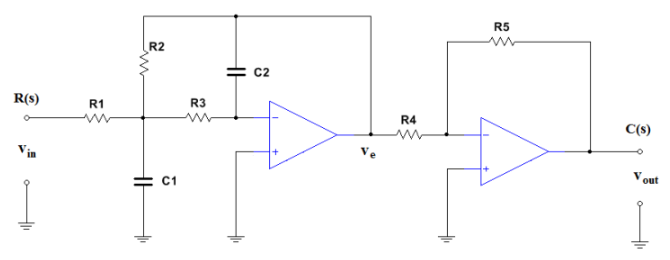
\includegraphics[width=0.5\textwidth]{media/sistema-segundo_orden}
		\caption{Circuito de 2do orden con Amplificadores Operacionales}
		\label{fig:sistema-segundoorden}
	\end{figure}
	
	Como se define en \cite{ogata2015} la función de transferencia de un sistema de segundo orden es una representación matemática que describe la relación entre la entrada y la salida de un sistema lineal e invariante en el tiempo en el dominio de la frecuencia, la cual nos permite describir y conocer los parámetros de los cuales depende el sistema y definen su comportamiento.
	
	Es por ello que para poder modelar la respuesta del sistema se tendrá en cuenta el modelo matemático de un sistema de segundo orden el cual se define en la ecuación \ref{eq:sistema-2do-orden} y que muestra los parámetros característicos de un sistema de 2do orden son:
	
	\begin{equation}
		H(s) = \frac{K \cdot \omega_n^2}{s^2 + 2\zeta\omega_n s + \omega_n^2}
		\label{eq:sistema-2do-orden}
	\end{equation}
	
	Donde: \\ 
	K: Es la ganancia del sistema \\
	$\omega_n$: Es la frecuencia natural no amortiguada \\
	$\zeta$: El factor de amortiguamiento del sistema \\
	
	Una vez definido el sistema de segundo orden para obtener la función de transferencia se debería buscar la relación definida en la ecuación \ref{eq:ft-1}
	
	\begin{equation}
		H(s) = \frac{C(s)}{V_i(s)}
		\label{eq:ft-1}
	\end{equation}
	
	Para la obtención de la función de transferencia se tomo como punto de referencia el punto de $V_e$ es cual servirá de nexo entre ambas etapas del circuito facilitando la obtención de la función de transferencia en el cual se hará uso de las diferentes técnicas para el análisis de sistemas como lo son las leyes de Kirchhoff y ley de ohm.
	
	Al relacionar las diferentes señales de entrada y salida se obtiene la siguiente función de transferencia.
	{\small
	\begin{equation}
		H(s) = \frac{R_2 R_5}{R_1 R_2 R_3 R_4 C_1 C_2 S^2 + (R_2 R_3 + R_1 R_3 + R_1 R_2)R_4 C_2 S + R_1 R_4}
		\label{eq:ft}
	\end{equation}
	}	
	
	Considerando la función de transferencia obtenida y el arreglo de resistencia equivalentes con igual magnitud, la ecuación \ref{eq:ft} se reduce a la siguiente expresión
	
	\begin{equation}
		H(s) = \frac{R^2}{R^4 C_1 C_2 S^2 + (3R^3 C_2)S + R^2}
		\label{eq:ft-reducida}
	\end{equation}
	
	Al comparar la ecuación \ref{eq:ft-reducida} con la ecuación \ref{eq:sistema-2do-orden} todavía es necesario modificar la función de transferencia obtenida, por lo que será necesario dividir a toda la ecuación por el factor $\frac{1}{R^2 C_1 C_2}$ al realizar esta operación se podrá obtener la siguiente función de transferencia.
	
	\begin{equation}
		H(s) = \frac{ \frac{1}{R^2C_1C_2]} }{ S^2 + \frac{3S}{RC_1} + \frac{1}{R^2C_1C_2}}
		\label{eq:ft-final}
	\end{equation}
	
	Ecuación de la cual se puede comprobar que la relación para la frecuencia natural será de: $\omega_n =\frac{1}{R \sqrt{C_1 C_2}}$ y el factor de amortiguamiento igual a $\zeta = \frac{3}{2} \sqrt{\frac{C_2}{C_1}}$ comprobando las relaciones especificadas para un sistema de 2do orden.
	
	\section{Calculo de $R C_1 y C_2$ según el polo asignado}
	\subsection{Caso Subamortiguado}
	
	Para el calculo de la resistencia R se tendrá en cuenta la función de transferencia reducida definida en \ref{eq:ft-final} y de la cual se usará el coeficiente del termino de primer grado para despejar el valor de la resistencia y el cual tendrá que evaluarse en función al valor del polo asignado.
	
	Para el polo simétrico ubicado en el plano complejo para $-1 \pm 8i$, se deberá realizar el producto de estos polos de forma que se obtenga la forma se una ecuación de 2do orden para poder realizar la comparación, para este caso se tiene que:
	\begin{equation}
		(s + 1 + 8j)(s + 1 - 8j) = s^2 + 2s + 65
		\label{eq:polo-subamortiguado}
	\end{equation}
	
	De la ecuación \ref{eq:polo-subamortiguado} se puede obtener que la relación $2\zeta \omega_n$ será igual 2 y de la cual se obtendrá el valor del factor de amortiguamiento $\zeta$ según la ecuación
	
	\begin{equation}
		\zeta = \frac{2}{2 \omega_n}
		\label{eq:factor-amortiguamiento}
	\end{equation}
	
	Y para la frecuencia natural o no amortiguada, se tiene la siguiente relación:
	
	\begin{equation}
		\omega_n = \sqrt{65} = 8.062
		\label{eq:frecuencia-natural}
	\end{equation}
	
	Finalmente obteniendo el valor de $\zeta$ reemplazando el valor de $\omega_n$ en la ecuación \ref{eq:factor-amortiguamiento}, será:
	
	\begin{equation}
		\zeta = \frac{2}{ 2 \omega_n} = 0.124
	\end{equation}
	
	Una vez definido el valor de los parámetros de un sistema de 2do orden se pueden calcular el valor de resistencia y capacitancias necesarias para establecer el sistema según las características definidas y el cual tendrán los siguientes valores asumiendo un valor de capacitancia $C_1 = 470\mu F \label{eq:sub-capacitancia-c1}$, se tiene: 
	
	\begin{align}
		R &=  7500\Omega \label{eq:sub-resistencia}\\
		C_2 &= 0.683 \mu F \approx 1 \mu F \label{eq:sub-capacitancia-c2}
	\end{align}
	
	Seguidamente para definir los parámetros de respuesta para el sistema, se define: \\
	
	\begin{align}
		T_p &= \frac{\pi}{\omega_d} \\
		T_s &= \frac{4}{\zeta \omega_n} \\
		T_r &= \frac{1.8}{\omega_n} \\
		M_p &= 100e^{ \frac{-\pi \zeta}{ \sqrt{1 - \zeta^2}} }
	\end{align}
	Donde :
	$T_p$ : Tiempo pico 
	$T_s$ : Tiempo de establecimiento 
	$T_r$ : Tiempo de crecimiento (relación aproximada)
	$M_p$ : Sobre pico
	
	Obteniendo para cada parámetro los siguientes valores numéricos o de magnitud para un determinado valor
	\begin{align}
		T_p &= 0.392s \\
		T_s &= 4 \\
		T_r &= 0.223s \\
		M_p &= 67.53\%
	\end{align}
	
	
	\subsection{Caso Sobreamortiguado}
	Para el caso del sistema sobreamortiguado de igual forma que el sistema subamortiguado para obtener los parámetros del sistema se hará uso de los polos asignados para el calculo de la función de 2do orden con la cual se definirán la frecuencia natural y el factor de amortiguamiento, esto se define de la siguiente forma
	\begin{equation}
		(s + 20.5)(s + 10.5) = s^2 + 31s + 215.25
		\label{eq:sobreamortiguado}
	\end{equation}
	
	De tal relación se determina que los valores de $\zeta$ y $\omega_n$ serán:
	
	\begin{align}
		\zeta &= 1.0564 \\
		\omega_n &= 14.671 
	\end{align}
	
	Obteniendo un valor de resistencia y capacitancia $C_2$ cuando $C_1 = 22 \mu F \label{eq:sobre-capacitancia-c1}$ 
	\begin{align}
		R = 2199.413 \Omega \approx 2.2K \Omega \label{eq:sobre-resistencia}\\ 
		C_2 = 10.913 \mu F \approx 10 \mu F \label{eq:sobre-capacitancia-c2}
	\end{align}	
	
	Finalmente para la obtención del tiempo de establecimiento para el caso de un sistema sobreamortiguado como se define en \cite{sistemas_segundo_orden}, se tiene:
	\begin{equation}
		T_s = \frac{2\zeta}{\omega_n}
		\label{eq:ts-sobreamortiguada}
	\end{equation}
	Para el caso de este sistema sobre amortiguado, se tendrá el siguiente valor calculado 
	$ T_s = 0.144s$ 
	
	\section{Desarrollo y gráficas en MATLAB}
	\subsection{Caso Subamortiguado}
	
	Respuesta al impulso unitario para el sistema sobre amortiguado con los polos simétricos en $ s = -1 \pm 8j$
	\begin{figure}[h]
		\centering
		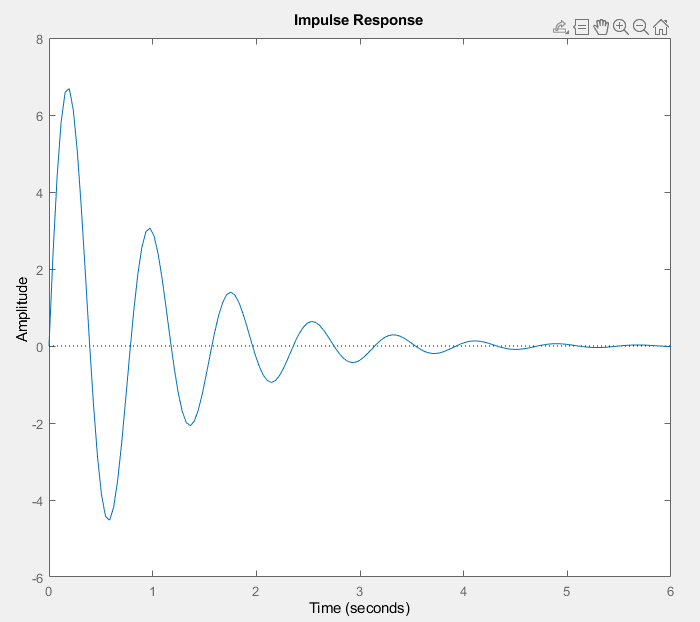
\includegraphics[width=0.3\textwidth]{media/sub-impulso}
		\caption{Respuesta al impulso unitario}
		\label{fig:sub-impulso}
	\end{figure}
	
	Respuesta frente al escalón unitario del sistema subamortiguado para el sistema previamente definido
	
	\begin{figure}[h]
		\centering
		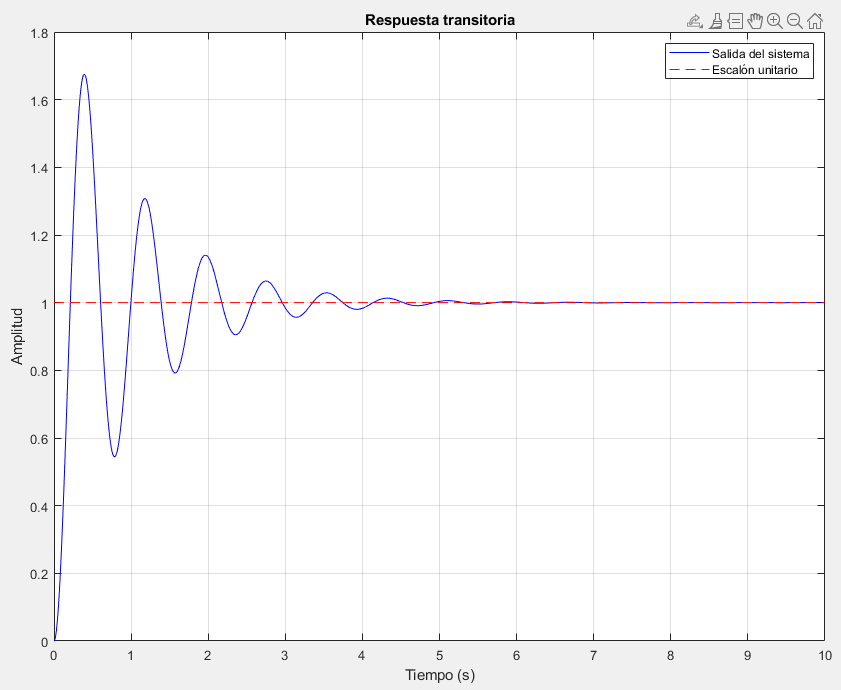
\includegraphics[width=0.3\textwidth]{media/sub-escalon}
		\caption{Respuesta al escalón unitario}
		\label{fig:sub-escalon}
	\end{figure}
	
	
	\subsection{Caso Sobreamortiguado}
	
	Respuesta al impulso unitario para el sistema sobre amortiguado para los polos definidos en $ s = -20.5, s = - 10.5$
	
	\begin{figure}[h]
		\centering
		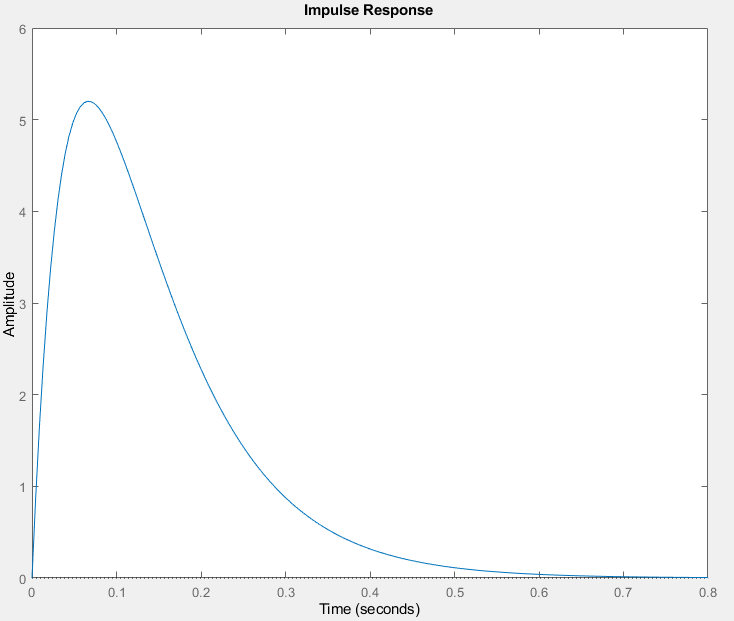
\includegraphics[width=0.3\textwidth]{media/sobre-impulso}
		\caption{Respuesta al impulso del sistema sobreamortiguado}
		\label{fig:sobre-impulso}
	\end{figure}
	Respuesta del sistema respecto a una entrada escalón unitario para los polos definidos previamente
	\begin{figure}[h]
		\centering
		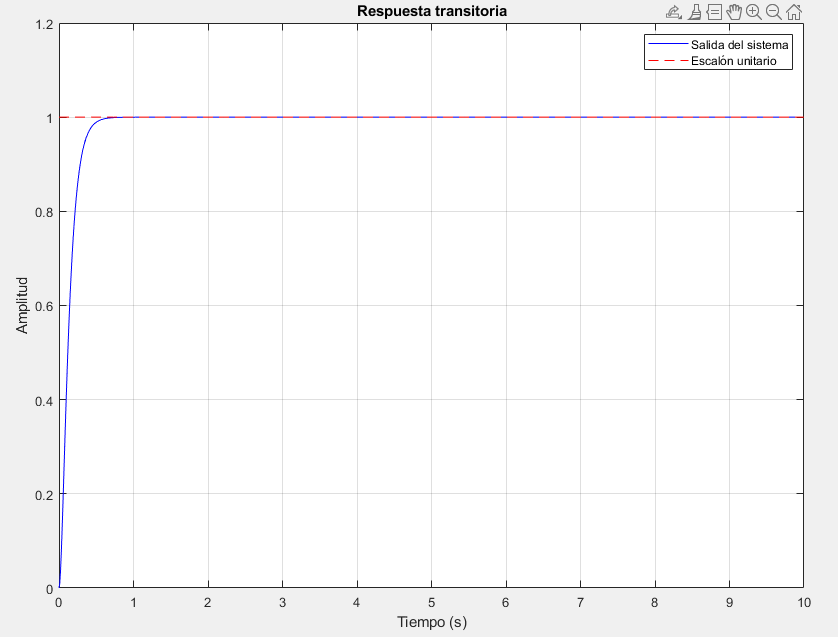
\includegraphics[width=0.3\textwidth]{media/sobre-escalon}
		\caption{Respuesta respecto a la entrada escalón unitario}
		\label{fig:sobre-escalon}
	\end{figure}
	
	\subsection{¿Qué significan las gráficas?}
	
	\textbf{Respuesta al impulso unitario (Caso subamortiguado)}
	En esta gráfica se observa la respuesta a un impulso unitario de un sistema subamortiguado con polos en $s = -1 \pm 8j$. La respuesta presenta oscilaciones antes de estabilizarse, lo cual es característico de un sistema subamortiguado. Estas oscilaciones indican que el sistema tiene un componente imaginario, que causa que el sistema oscile con una amplitud que decrece exponencialmente en el tiempo.
	
	\textbf{Respuesta al escalón unitario (Caso subamortiguado)}
	Aquí se muestra la respuesta a un escalón unitario de un sistema subamortiguado. Se observa un comportamiento similar al de la respuesta al impulso, pero en este caso, el sistema tiende hacia un valor constante a largo plazo, tras experimentar oscilaciones iniciales. La presencia de esas oscilaciones, aunque amortiguadas, sigue siendo notable, y el sistema alcanza el valor deseado tras varias fluctuaciones.
	
	\textbf{Respuesta al impulso del sistema sobremortiguado}
	Esta gráfica corresponde a la respuesta a un impulso unitario de un sistema sobremortiguado con polos en 
	$ s = -20.5, s = -10.5$. A diferencia del caso subamortiguado, no se presentan oscilaciones. La respuesta se eleva rápidamente y luego desciende de manera suave y continua hasta alcanzar la estabilización. Esto es característico de un sistema sobremortiguado, donde los polos son reales y distintos, lo que evita las oscilaciones.
	
	\textbf{Respuesta al escalón unitario del sistema sobremortiguado}
	Esta gráfica muestra la respuesta a un escalón unitario de un sistema sobremortiguado. El sistema responde rápidamente y se ajusta al valor final sin presentar oscilaciones, pero lo hace de manera más lenta que un sistema críticamente amortiguado. La curva se aproxima suavemente a su valor final y se estabiliza.
	
	\section{Comprobación de los valores teóricos con los simulados}
	\subsection{Caso del sistema subamortiguado}
	\subsubsection{Frecuencia natural no amortiguada $\omega_n$}
	En el caso del sistema subamortiguado la frecuencia natural o no amortiguada este valor se define a partir de la ecuación de 2do orden y la cual esta descrita mediante el termino independiente del denominador como se describe en la ecuación \ref{eq:sistema-2do-orden} y cuyo valor para un sistema subamortiguado será de $\omega_n = 8.06$
	
	\subsubsection{Frecuencia amortiguada $\omega_d$}
	
	La frecuencia natural amortiguada se define como el producto de la frecuencia natural por la raiz cuadrada de uno menos el factor de amortiguamiento al cuadrado y es el parámetro que establece en que medida el sistema oscilara antes de llegar a la estabilidad, de forma matemática su equivalencia es:
	\begin{align}
		\omega_d &= \omega_n \sqrt{1 - \zeta^2} \\
		\omega_d &= 8
	\end{align}
	
	\subsubsection{Factor de amortiguamiento $\zeta$}
	El factor de amortiguamiento para el sistema, será de: 
	\begin{equation}
		\zeta = 0.124
		\label{eq:sub-factor-amortiguamiento}
	\end{equation}
	Y se define como la razón entre el coeficiente del termino de grado 1 de la ecuación característica de 2do orden, respecto a la doble de la frecuencia natural.
	
	\subsubsection{Atenuación $\sigma$}
	La atenuación de un sistema se define como el producto de la frecuencia natural por el factor de amortiguamiento y describe en que medida las oscilaciones se irán atenuando.
	
	\begin{equation}
		\sigma = \omega_n \zeta
		\label{eq:atenuacion}
	\end{equation}
	
	Haciendo uso de la ecuación \ref{eq:atenuacion} el valor de la atenuación, será:
	
	\begin{equation}
		\sigma = 1
	\end{equation}
	
	\subsection{Caso del sistema sobreamortiguado}
	
	Para el caso del un sistema sobreamortiguado las ecuaciones para definir sus parámetros no variaran a los de un sistema subamortiguado debido a que estos valores se encuentra definidos en función a la ecuación general para los sistemas de 2do orden, por lo tanto se tendrá las siguientes relaciones para ello.
	
	\subsubsection{Frecuencia natural no amortiguada $\omega_n$}
	
	La frecuencia natural será $ \omega_n = 14.67$
	
	\subsubsection{Frecuencia amortiguada $\omega_d$}
	La frecuencia natural amortiguada debido a que $\zeta$ es mayor a 1, indetermina este valor haciendo que no existe gracias a la \textbf{sobreamortiguación del sistema}
	
	\subsubsection{Factor de amortiguamiento $\zeta$}
	El factor de amortiguamiento para este tipo de sistema será:
	\begin{equation}
		\zeta = 1.056
		\label{eq:sobre-factor-amortiguamiento}
	\end{equation}
	
	\subsubsection{Atenuación $\sigma$}
	Finalmente la atenuación equivaldrá a:
	\begin{equation}
		\sigma = 15.5
	\end{equation}
	
	El cual es un valor mayor a la frecuencia natural lo cual es un indicador de que las oscilaciones del sistema se atenuarán a una mayor velocidad y razón de cambio.
	
	\section{Diseño del circuito}
	Los valores de resistencia y capacitancia para la planta de segundo orden definida se hallaron para cada tipo de sistema teniendo en cuenta los valores de R y C más cercanos a los valores comerciales para estos elementos y cuyas magnitudes no sean muy elevadas o mínimas debido a las condiciones de polarización para los circuitos integrados a utilizar.
	
	Las magnitudes de los valores a utilizar se definen en \ref{eq:sub-resistencia}, \ref{eq:sub-capacitancia-c1}, \ref{eq:sub-capacitancia-c2} para el sistema subamortiguado y en \ref{eq:sobre-resistencia}, \ref{eq:sobre-capacitancia-c1},\ref{eq:sobre-capacitancia-c2} para el sistema sobreamortiguado
	
	\subsection{Sistema subamortiguado}
	Planta para el sistema de 2do orden subamortiguado definido por 2 etapas compuestas por amplificadores operacionales para definir cada bloque, este sistema debido a la existencia de las 2 capacitancias, se convertirá en un sistema de 2do orden el cual estará caracterizado por diferentes parámetros comunes y relativos al tiempo de respuesta.
	\begin{figure}[h]
		\centering
		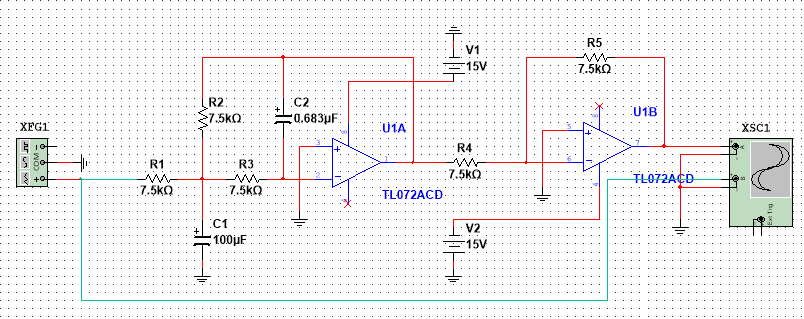
\includegraphics[width=0.4\textwidth]{media/sistema-subamortiguado}
		\caption{Planta de 2do orden subamortiguada}
		\label{fig:sistema-subamortiguado}
	\end{figure}
	
	\subsection{Respuesta del sistema cuando $V_i$ es un tren de impulsos}
	
	\begin{figure}[h]
		\centering
		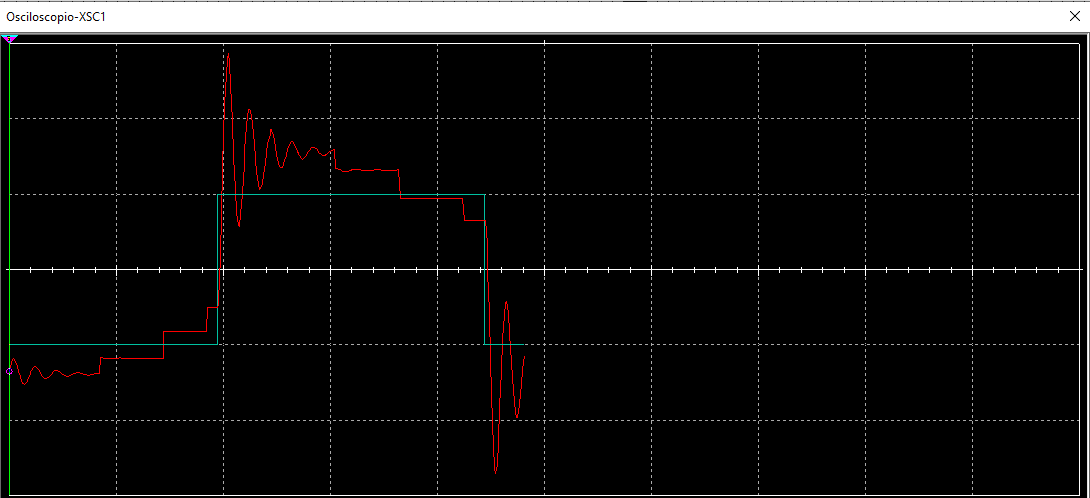
\includegraphics[width=0.4\textwidth]{media/sub-tren-impulsos}
		\caption{Respuesta del sistema frente a una entrada escalón unitario}
		\label{fig:sub-tren-impulsos}
	\end{figure}
	
	\subsection{Sistema sobreamortiguado}
	Planta para el sistema de 2do orden sobreamortiguado
	
	\begin{figure}[h]
		\centering
		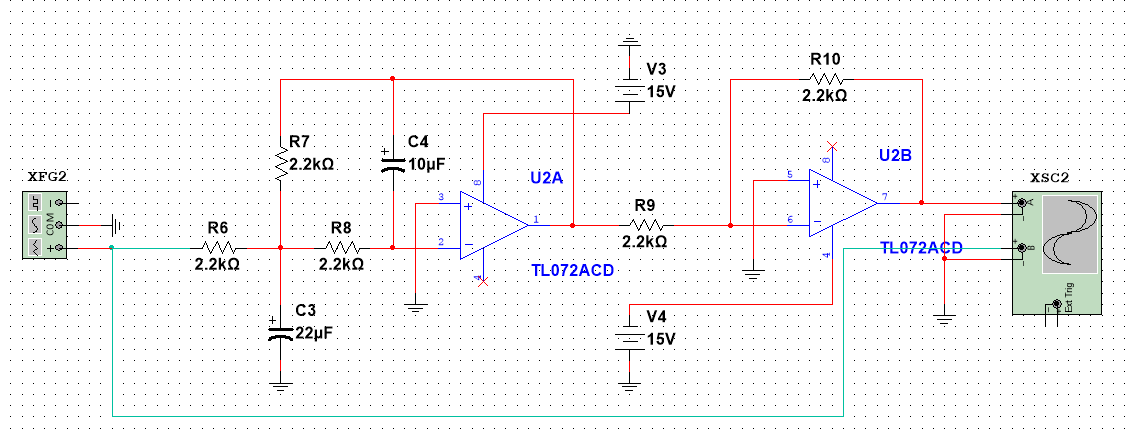
\includegraphics[width=0.4\textwidth]{media/sistema-sobreamortiguado}
		\caption{Sistema de 2do orden sobreamortiguado}
		\label{fig:sistema-sobreamortiguado}
	\end{figure}
	
	\subsection{Respuesta del sistema cuando $V_i$ es un tren de impulsos}
	
	\begin{figure}[h]
		\centering
		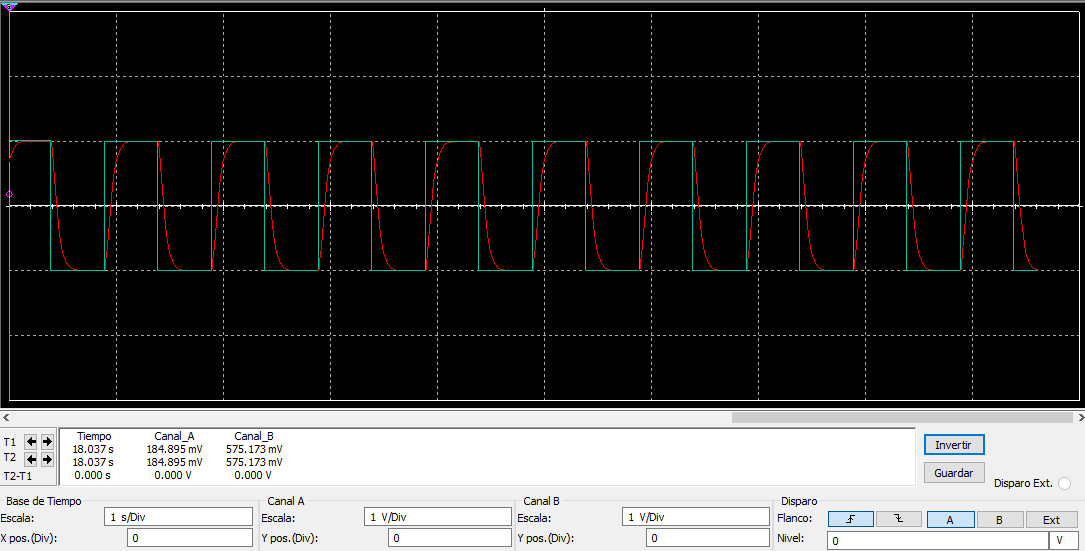
\includegraphics[width=0.4\textwidth]{media/sobre-tren-impulsos}
		\caption{Respuesta del sistema frente a una entra escalón unitario}
		\label{fig:sobre-tren-impulsos}
	\end{figure}
	
	\bibliographystyle{IEEEtran}
	\bibliography{biblio}
\end{document}
